\section{Blockchain}
In diesem Grundlagen Kapitel soll ein Verständnis für die unterschiedlichen Begriffe und Verfahren der Blockchain Technologie etabliert werden. Beginnend mit einer allgemeinen Definition des Begriffs Blockchain, werden die verschiedenen Arten von \ac{dlt} im Detail betrachtet und definiert. Eine Abgrenzung zu Kryptowährungen soll zeigen, dass Blockchain nicht gleich Kryptowährungen bedeutet. In Kapitel 2.4 wird der technologische Hintergrund erörtert und abschließend soll eine Auflistung der vorhandenen \ac{dlt} die aktuelle Herstellerlandschaft zeigen.

\subsection{Definition}
Unter dem Begriff Blockchain wird eine Technologie verstanden, die eine erweiterbare Liste von Datensätzen bildet. Jeder Eintrag in dieser Liste wird Block genannt und ist durch kryptographische Methoden untereinander verkettet. Als Inhalt besitzt jeder Block einen kryptographischen Hashwert des vorhergehenden Blocks, sowie einen Zeitstempel und die eigentlichen Daten.\cite[Vgl.]{narayanan2016bitcoin}\\
Technisch ist eine Blockchain also eine Art dezentrale Datenbank. Das Netzwerk aus Teilnehmern der Blockchain entscheidet im Konsens welcher Block (Datensatz) valide ist und der Gesamtmenge an Blöcken (Datenbank) angehangen wird. Zur Konsensbildung werden spezielle Algorithmen verwendet, um einen sog. byzantinischen Fehler zu verhindern. Durch die Vielzahl der Teilnehmer kann das mögliche Fehlermodell bei der Konsensbildung sehr komplex und schwer zu erfassen sein. Darauf beziehen sich byzantinische Fehler und die vorhandenen Lösungsansätze.\\
Der Oberbegriff \acf{dlt} wird in diesem Kontext gleichermaßen Synonym verwendet. Jedoch muss nicht zwingend jedes \glqq Distributed Ledger\grqq{} eine Blockchain als technische Grundlage verwenden. Viele unterschiedliche Ansätze werden aktuell in der Forschung und freien Marktwirtschaft erprobt und auf ihre Eigenschaften hin untersucht.\\
Das hohe Maß an Sicherheit, welches mit dem Begriff Blockchain assoziert wird, wird durch die Signierung der Blöcke und Transaktionen mit dem Public-Key-Verfahren garantiert. Auf dieses kryptographische Verfahren wird in Kapitel \ref{tec_bkgrnd_sec} näher eingegangen.\cite[Vgl.]{Mitschele2018}

\subsection{Arten von \acl{dlt}}


\subsubsection{Blockchain}
\begin{figure}[h!]
	\centering
	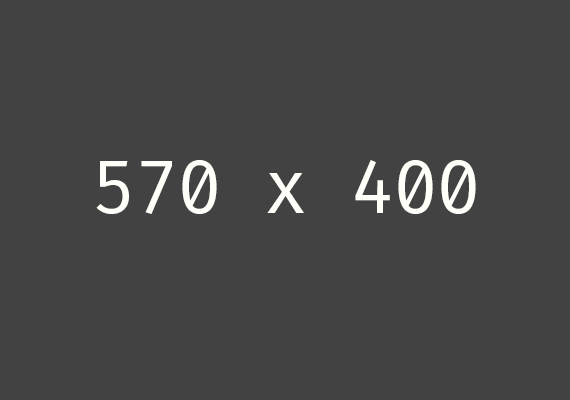
\includegraphics[width=1.0\linewidth]{pictures/placeholder_half_page}
	\caption[Placeholder Half Page]{Placeholder Half Page}
	\label{fig:placeholder_half_page}
\end{figure}


\subsubsection{Tangle}


\subsubsection{Hash Graph}
\begin{figure}[h!]
	\centering
	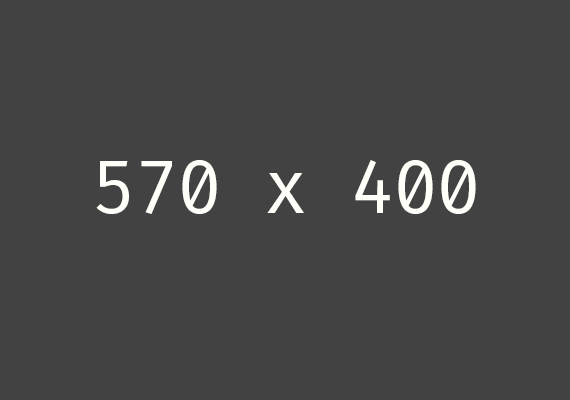
\includegraphics[width=1.0\linewidth]{pictures/placeholder_half_page}
	\caption[Placeholder Half Page]{Placeholder Half Page}
	\label{fig:placeholder_half_page}
\end{figure}


\subsubsection{Public}


\subsubsection{Private}


\subsubsection{Consortium}


\subsection{Abgrenzung Kryptowährungen}


\subsection{Technologischer Hintergrund}


\subsubsection{Sicherheit} \label{tec_bkgrnd_sec}


\paragraph{Public-Key Authorization}
\begin{figure}[h!]
	\centering
	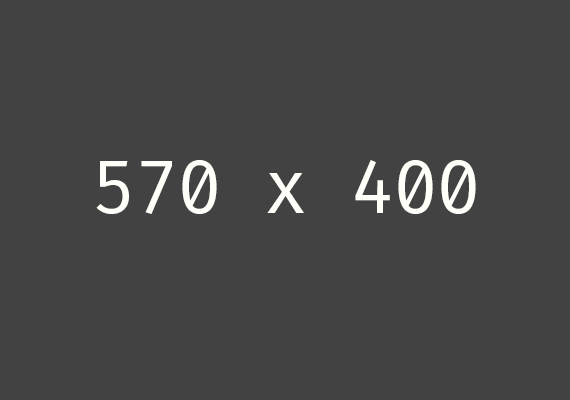
\includegraphics[width=1.0\linewidth]{pictures/placeholder_half_page}
	\caption[Placeholder Half Page]{Placeholder Half Page}
	\label{fig:placeholder_half_page}
\end{figure}


\paragraph{Hashing Algorithmus}


\subsubsection{Consensus Algorithmus}
\begin{figure}[h!]
	\centering
	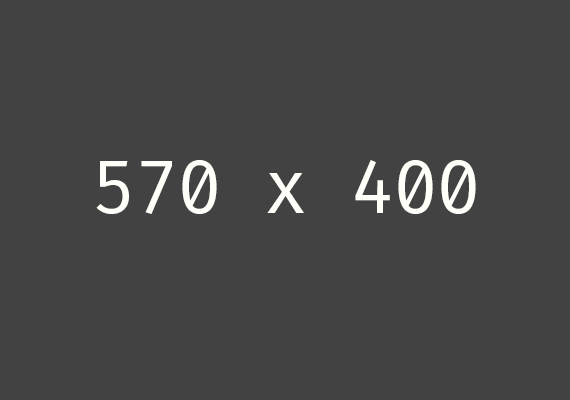
\includegraphics[width=1.0\linewidth]{pictures/placeholder_half_page}
	\caption[Placeholder Half Page]{Placeholder Half Page}
	\label{fig:placeholder_half_page}
\end{figure}


\paragraph{Proof-of-Work}
\begin{figure}[h!]
	\centering
	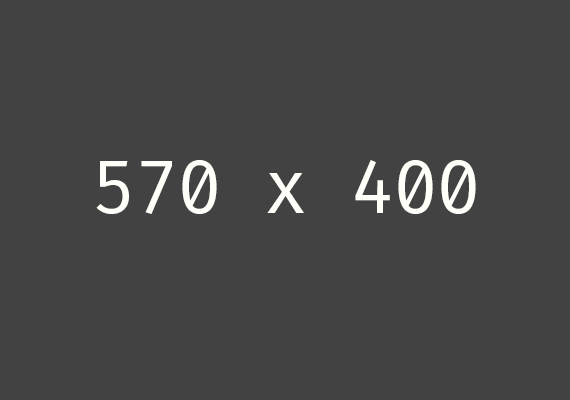
\includegraphics[width=1.0\linewidth]{pictures/placeholder_half_page}
	\caption[Placeholder Half Page]{Placeholder Half Page}
	\label{fig:placeholder_half_page}
\end{figure}


\paragraph{Proof-of-Stake}
\begin{figure}[h!]
	\centering
	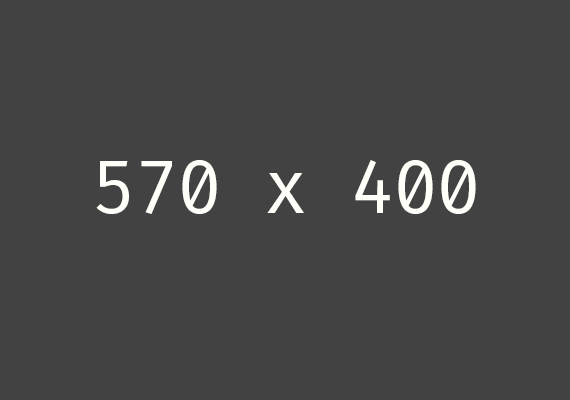
\includegraphics[width=1.0\linewidth]{pictures/placeholder_half_page}
	\caption[Placeholder Half Page]{Placeholder Half Page}
	\label{fig:placeholder_half_page}
\end{figure}


\paragraph{Delegated Proof-of-Stake}


\subsubsection{Peer-to-Peer Netzwerke}
\begin{figure}[h!]
	\centering
	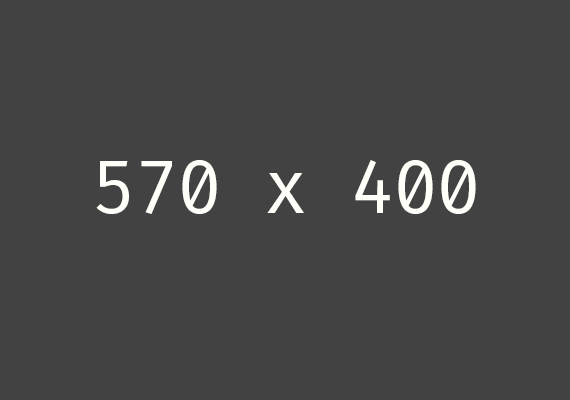
\includegraphics[width=1.0\linewidth]{pictures/placeholder_half_page}
	\caption[Placeholder Half Page]{Placeholder Half Page}
	\label{fig:placeholder_half_page}
\end{figure}


\subsubsection{Distributed Computing}


\subsection{Vorhandene Distributed Ledger}


\subsubsection{Bitcoin}


\subsubsection{Ethereum}


\subsubsection{IOTA}


\subsubsection{Ripple}


\subsubsection{IBM Bluemix}


\subsubsection{Microsoft Azure}


\subsubsection{Hyperledger Fabric}


\newpage